\documentclass[letterpaper, 11pt]{article}
\usepackage{comment} % enables the use of multi-line comments (\ifx \fi) 
\usepackage{fullpage} % changes the margin
\usepackage{fancyhdr} % for footer
\usepackage[UKenglish]{isodate}% http://ctan.org/pkg/isodate for date format
\usepackage{float}%force tables/figs into certain placement
\usepackage{changepage}%for dichotomous key
\usepackage{graphicx}%for figures
\usepackage{caption}%for figures
\usepackage{subcaption}%for figures
\usepackage{hyperref}%for hyperlinks
\usepackage{multicol}% for making list span multiple columns
\usepackage[font=small,labelfont=bf]{caption}%for captions
\renewcommand{\headrulewidth}{0pt}
\def\labelitemi{--}
\pagestyle{fancy}

\lhead{}
\chead{}
\rhead{}
\lfoot{ENT 432 (Fall 2016) - Penn State}
\cfoot{}
\rfoot{\thepage}
\renewcommand{\footrulewidth}{0.4pt}
\title{Unit 5 - Non-hexapod Arthropoda}
\author{Andrew R. Deans and Istv\'an Mik\'o}
\begin{document}
\cleanlookdateon %removed ordinal date
\maketitle
\thispagestyle{fancy}
\section{Lecture}
In this unit we learn about major non-hexapod arthropod lineages---\textbf{Chelicerata} (spiders, mites, scorpions, and their relatives), \textbf{Myriapoda} (centipedes, millipedes, and their relatives), and some non-hexapod \textbf{Pancrustacea} (pillbugs, brine shrimp, and their relatives---including our collective understanding of their natural histories and hypotheses of their evolutionary history relative to other arthropods.

\subsection*{Taxa to know}
Familiarize yourself with the following taxon names, which refer to organisms you are likely to encounter in the northeastern USA. Can you describe how these arthropods live (natural history) and roughly how diverse they are? Do you know how they're related to one another? Could you identify one by sight?

\begin{multicols}{2}
\begin{enumerate} 
\item{Acari}
\item{Amphipoda}
\item{Arachnida}  
\item{Araneae}  
\item{Chelicerata} 
\item{Chilopoda}
\item{Diplopoda}
\item{Isopoda}  
\item{Myriapoda}
\item{Onychophora} 
\item{Opiliones}  
\item{Pancrustacea} 
\item{Pseudoscorpiones} 
\item{Scorpiones}
\item{Xenocarida (no specimens)}  
\end{enumerate}
\end{multicols}

\subsection*{Big picture questions}
\noindent{}We covered more taxa than those in the list above. Was there one that stood out to you as especially compelling? Can you spell it correctly and describe its relevance to our understanding of evolution, behavior, and morphology?\\

\noindent{}What was the first terrestrial arthropod? How do we know it was terrestrial?\\ 

\noindent{}Revisit our discussion of the phenotypes that make an organism an arthropod. Now consider their diversity relative to other metazoans: vertebrates, annelids, nematodes, \textit{etc}. What phenotypes would you consider ``key innovations''? Why is Arthropoda orders of magnitude more diverse than its sister lineage?\\

\section{Lab}

\subsection*{Introduction}
You should have a relatively firm grasp of arthropod anatomy at this point. It's time to start looking at specimens in the contexts of taxonomy and evolution. In this lab we will examine a few fossils, to get a sense of how much (or how little) information they provide. We will also look at specimens of velvet worms (Onychophora), the putative sister to Arthropoda, and non-insect arthropods. Based on your observations of their morphologies, how are insects related to these other arthropods? After this lab do you think you could recognize any of these taxa in the wild? We will focus primarily on arthropods you can find in Pennsylvania. 

\subsection*{Materials}
\begin{itemize}
\item specimens (provided)
\item fine forceps, probes (provided)
\item sorting tray, watch glasses, gloves, safety glasses, glycerol, ethanol (provided)
\item pencil/paper for sketches
\end{itemize}

\subsection*{Safety}
We will be working with sharp tools. Wear your personal protective gear at all times. Specimens are to be returned to their vials after lab, and glycerine and ethanol will be collected for proper disposal or reuse.

\subsection*{Methods}
Working with a partner, organize your space, specimens, tools, and microscope. Use your probe and forceps to manipulate the specimen. In this lab, however, we will not be dissecting specimens (unless otherwise noted). You can start anywhere in the handout.

\subsection{Onychophora (velvet worms)}
These organisms are thought to be sister to Arthropoda. Can you see any shared, derived characters (Figure \ref{fig:onych}) between onychophorans and arthropods? What features indicate that these creatures are definitely \textit{not} Arthropoda (\textit{i.e.}, how would you write the diagnosis)? \vspace{3cm}

\begin{figure}[ht!]
  \centering
    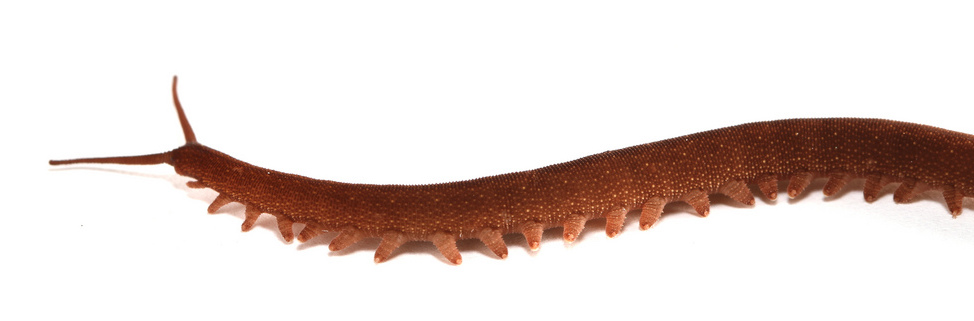
\includegraphics[width=0.8\textwidth]{onych}
  \caption{Photo (CC BY-NC-SA 2.0) by Yonatan Monk: \url{https://flic.kr/p/85z27d}}.
  \label{fig:onych}
\end{figure}

\subsection{Chelicerata}
These arthropods generally share the following characters: 
\begin{itemize}
\item antennae absent (though anteriormost pair of legs often antenniform)
\item 6 pairs of uniramous appendages: chelicerae (mouthparts) + pedipalps + 4 pairs of legs
\item 2 tagmata: prosoma (cephalothorax) and opisthosoma (abdomen)
\end{itemize}
The most diverse group of chelicerates is Arachnida, which includes all the terrestrial species of Chelicerata. We will examine specimens of the taxa listed below. Can you see the diagnostic characters clearly? If you saw any of these specimens in a lab practical could you name it (with correct spelling), describe a diagnostic feature, and/or describe its natural history?

\subsubsection*{Araneae (spiders)}
\begin{itemize}
\item chelicerae fang-like (Figure \ref{fig:fang})
\item anteriormost pair of legs not antenniform
\item pedipalps not chelate (\textit{i.e.}, pincer/claw-shaped), rarely stouter than legs
\item opisthosoma not obviously segmented (except rarely)
\item opisthosoma attached to prosoma via narrow constriction (Figure \ref{fig:spider})
\item spinnerets present posteroventrally on opisthosoma, but no tail-like structure (telson)
\end{itemize}
Why do spiders have a constricted ``waist''? What are fang-like chelicerae adapted for? Can you predict how they're used?\vspace{3cm}

\begin{figure}[ht!]
    \centering
    \begin{subfigure}[ht!]{0.25\textwidth}
        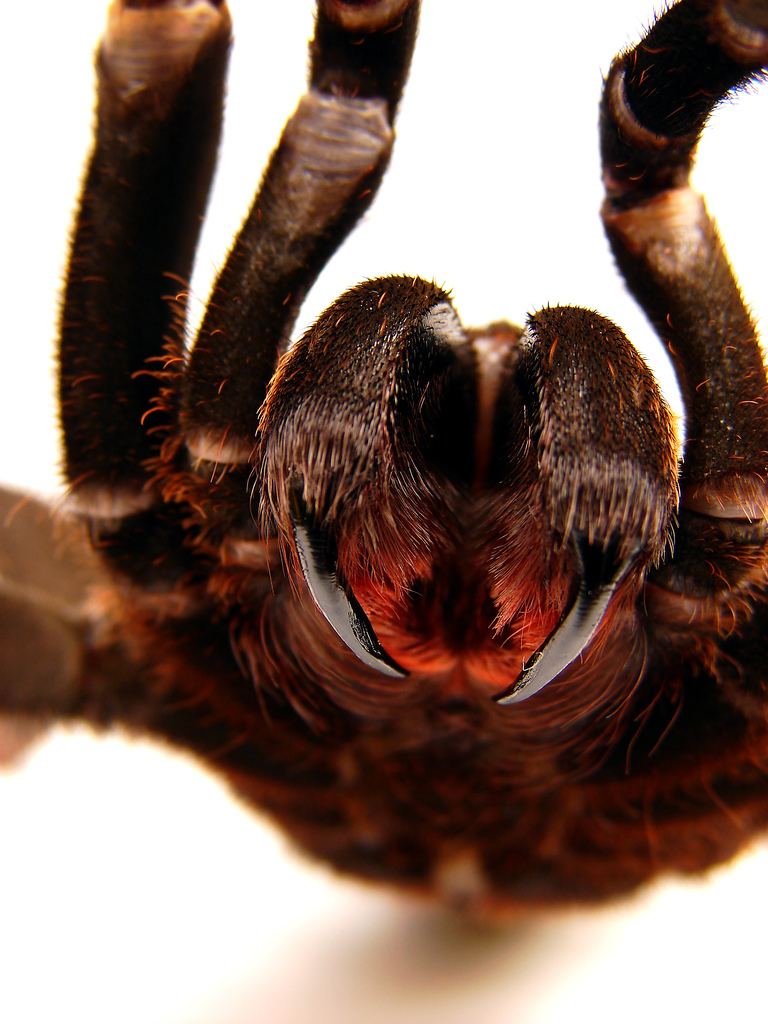
\includegraphics[width=\textwidth]{fang}
        \caption{Chelicerae. Photo (CC BY-SA 2.0) by Matt Reinbold: \url{https://flic.kr/p/2Bxryh}}
        \label{fig:fang}
    \end{subfigure}
    ~ %add desired spacing between images, e. g. ~, \quad, \qquad, \hfill etc. 
      %(or a blank line to force the subfigure onto a new line)
    \begin{subfigure}[ht!]{0.65\textwidth}
        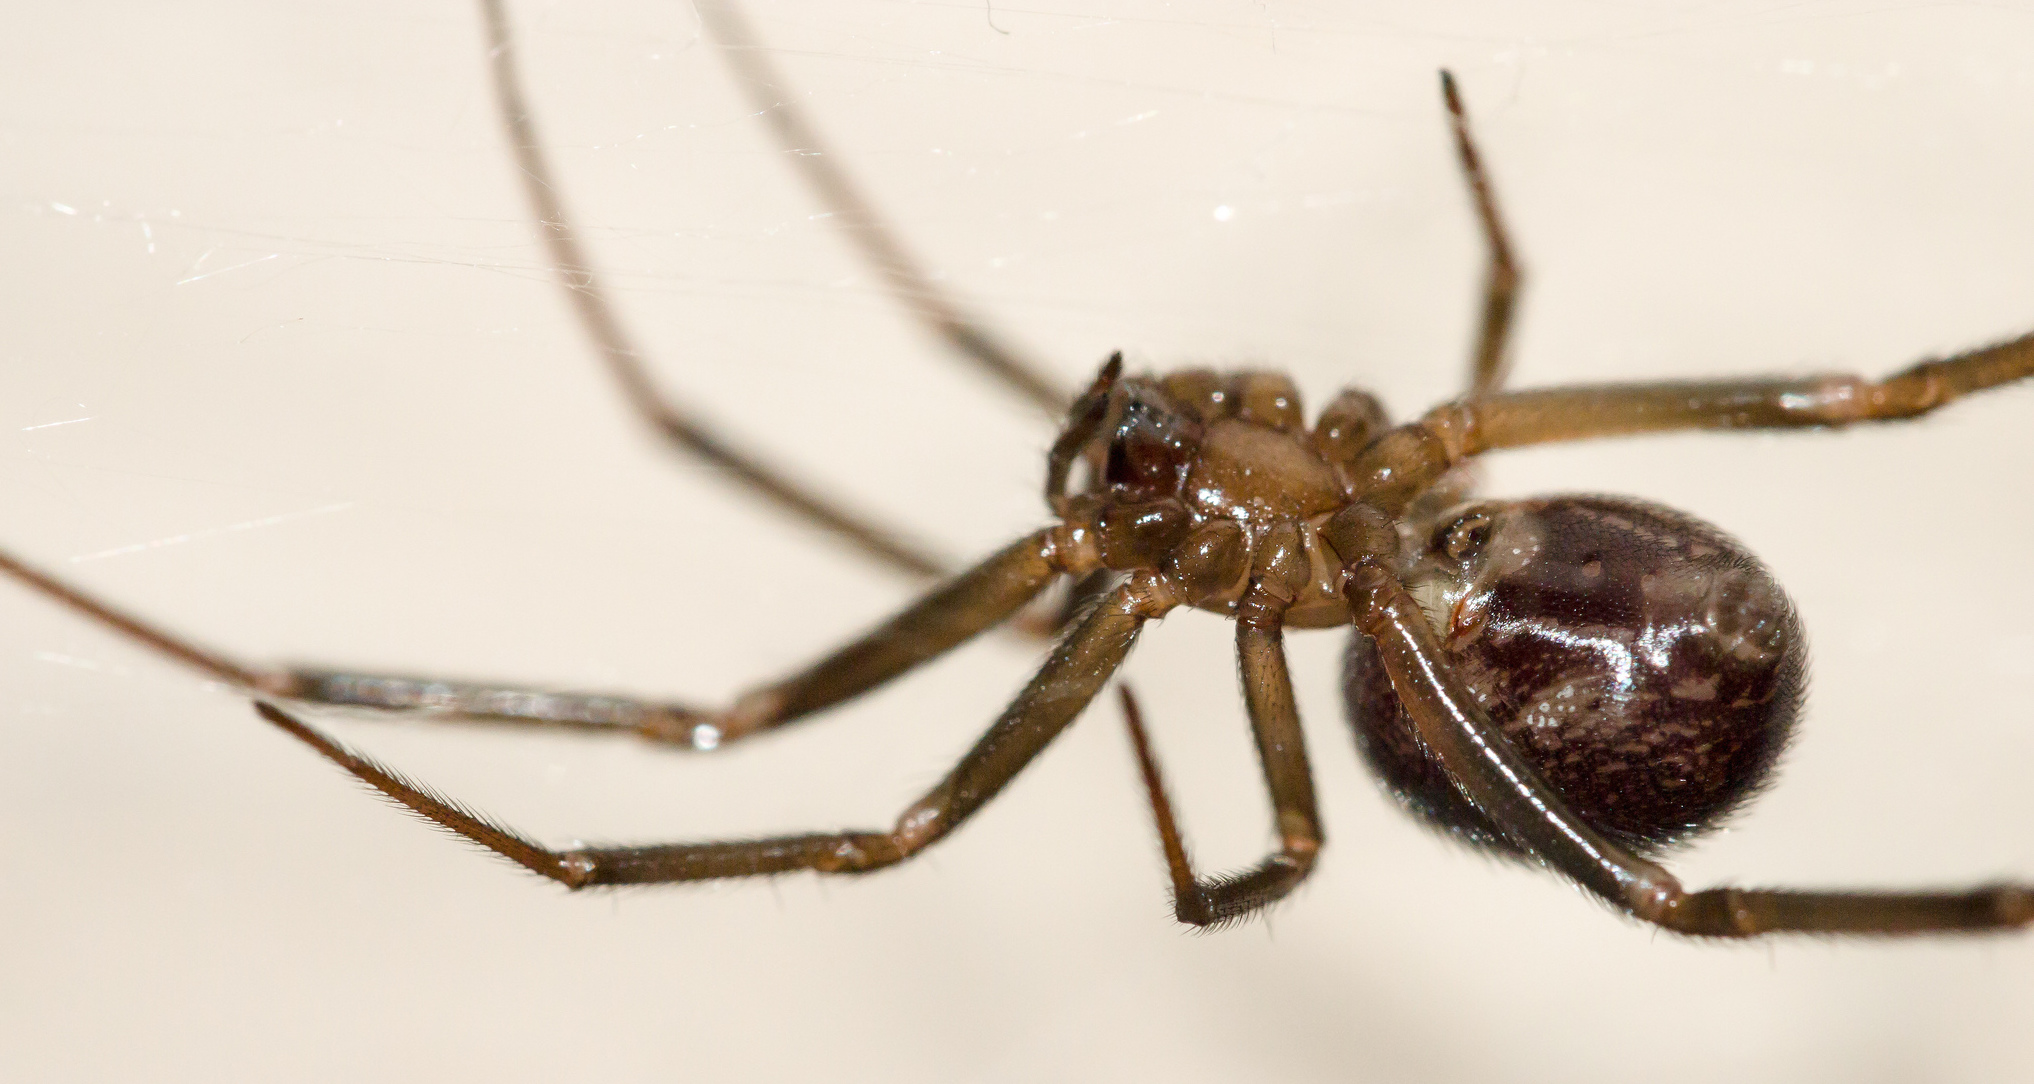
\includegraphics[width=\textwidth]{spider}
        \caption{Ventral habitus. Photo (CC BY-SA 2.0) by James E. Petts: \url{https://flic.kr/p/fJqUsE}}
        \label{fig:spider}
    \end{subfigure}
    \caption{Spiders (Araneae)}\label{fig:spiders}
\end{figure}

\subsubsection*{Acari (mites, ticks)}
\begin{itemize}
\item opisthosoma not segmented (See Figure \ref{fig:mites})
\item opisthosoma broadly joined to prosoma, no tail-like structure (telson)
\item young instars with 3 pairs of legs, adults with 4
\item pedipalps not chelate, not thicker than legs
\item mouthparts usually project anteriorly, chelicerae not chelate
\item usually very small (0.08--10 mm body length)
\end{itemize}
The apparent lack of segmentation is a diagnostic character. Can you see any evidence that these arthropods have segments? Based on their body shape and size, and especially their mouthpart morphology, can you make predictions or generalizations about their natural history?\vspace{5cm}

\begin{figure}[ht!]
    \centering
    \begin{subfigure}[ht!]{0.5\textwidth}
        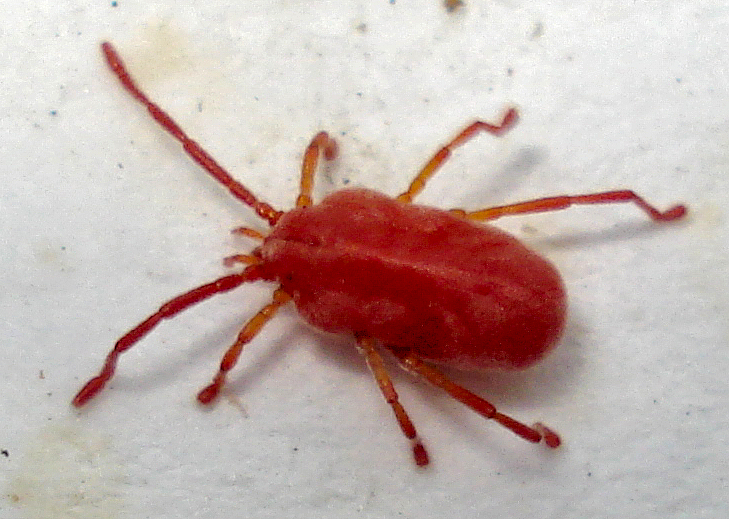
\includegraphics[width=\textwidth]{mite1}
        \caption{Dorsal habitus. Photo (CC BY 2.0) by Mick E. Talbot: \url{https://flic.kr/p/55WxVw}}
        \label{fig:mite1}
    \end{subfigure}
    ~ %add desired spacing between images, e. g. ~, \quad, \qquad, \hfill etc. 
      %(or a blank line to force the subfigure onto a new line)
    \begin{subfigure}[ht!]{0.4\textwidth}
        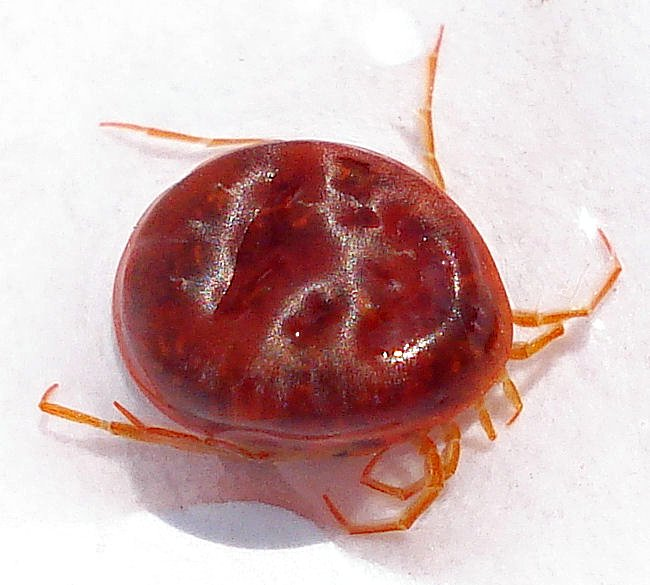
\includegraphics[width=\textwidth]{mite2}
        \caption{Dorsal habitus. Photo (CC BY 2.0) by Mick E. Talbot: \url{https://flic.kr/p/6s36QX}}
        \label{fig:mite2}
    \end{subfigure}
    \caption{Mites (Acari).} \label{fig:mites}
\end{figure}

\subsubsection*{Opiliones (harvestmen, daddy-longlegs)}
\begin{itemize}
\item chelicerae chelate
\item opisthosoma segmented, broadly joined to prosoma, without tail-like structure (telson) (Figures \ref{fig:opiliones1}--\ref{fig:opiliones2})
\item body ovoid; body  \textless7 mm long usually, with leg span up to 160 mm
\item pedipalp morphology variable: usually thinner than legs, sometimes raptorial 
\end{itemize}

\begin{figure}[ht!]
  \centering
    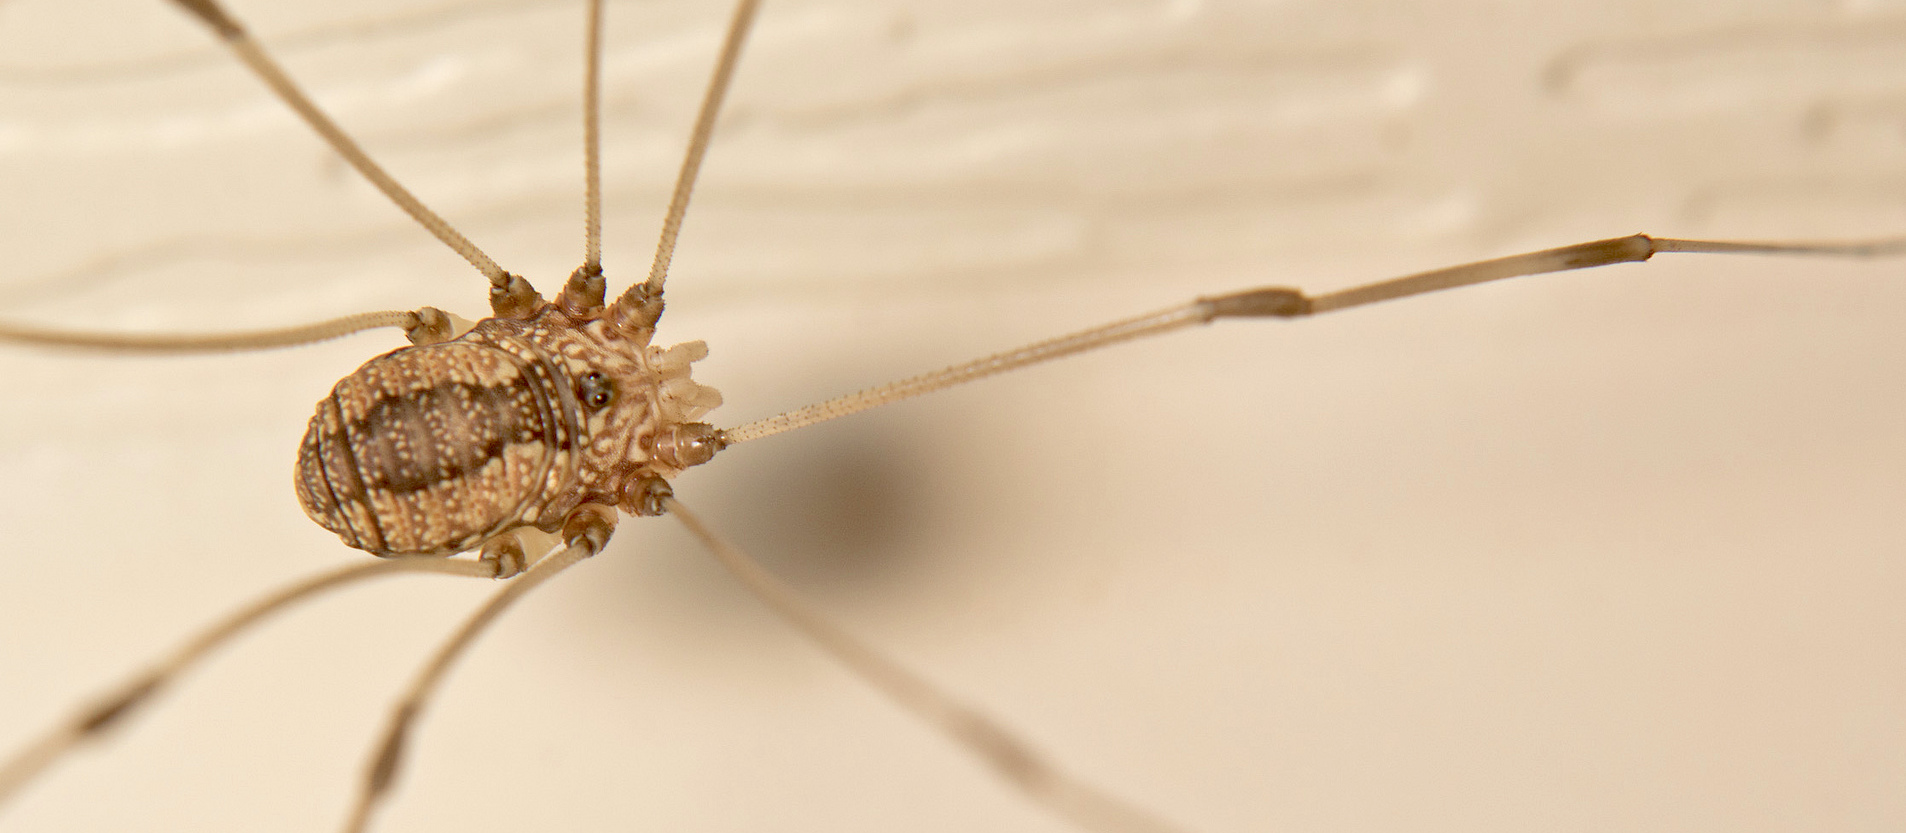
\includegraphics[width=0.7\textwidth]{opiliones1}
  \caption{Opiliones. Photo (CC BY-SA 2.0) by Gordon: \url{https://flic.kr/p/bVW3Yp}}
  \label{fig:opiliones1}
\end{figure}

\begin{figure}[ht!]
  \centering
    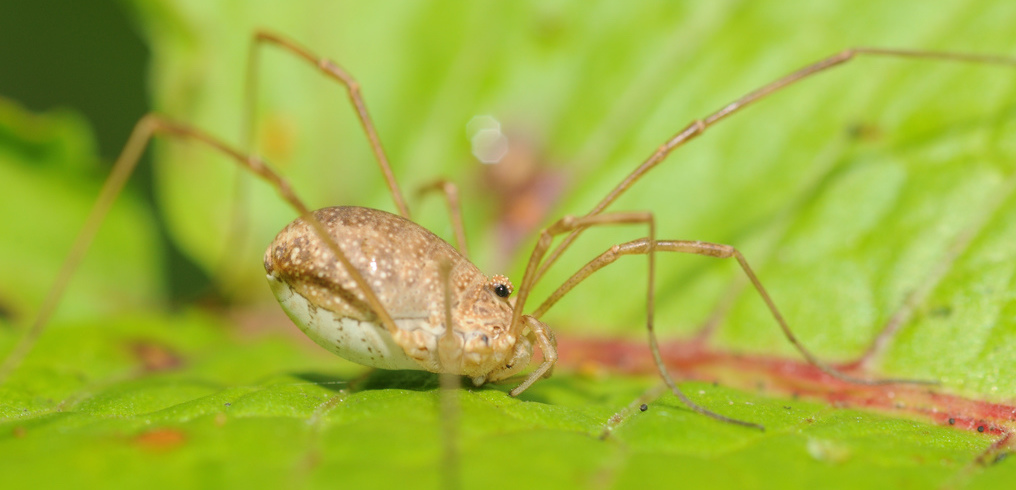
\includegraphics[width=0.7\textwidth]{opiliones2}
  \caption{Opiliones. Photo (CC BY 2.0) by Thomas Bresson: \url{https://flic.kr/p/6ytEzH}}
  \label{fig:opiliones2}
\end{figure}
\noindent{}Like all arachnids, Opiliones do not have antennae. Can you find an appendage that serves a similar function? Given the variation in pedipalp morphology across Opiliones, what would you predict is the function of these appendages?\vspace{3cm}

\subsubsection*{Scorpiones (scorpions)}
\begin{itemize}
\item chelicerae chelate
\item pedipalps long, chelate, and usually at least as thick as legs (Figure \ref{fig:scorpion})
\item anteriormost pair of legs used for walking (\textit{i.e.}, not antenniform)
\item opisthosoma segmented, broadly joined to prosoma; tail-like posteriorly (tail = telson)
\item telson with venom gland and sting present
\item 2nd segment of opisthosoma with comblike organs (pectines) ventrally 
\end{itemize}

\begin{figure}[ht!]
  \centering
    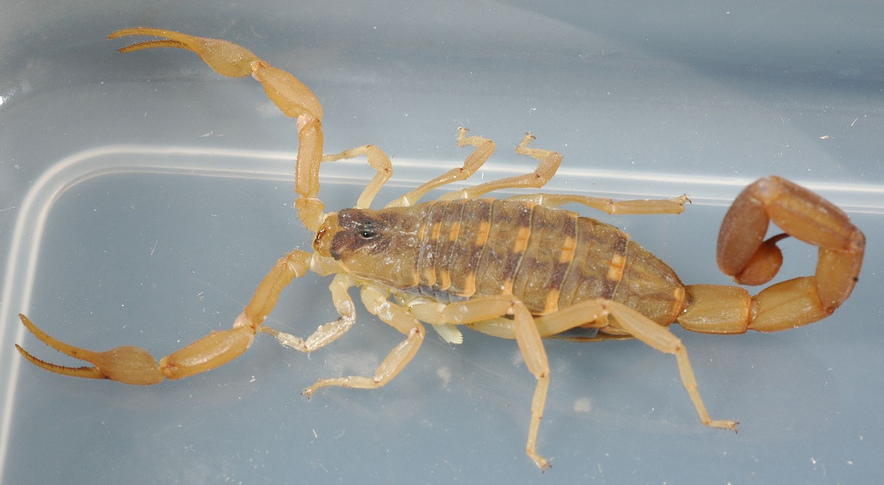
\includegraphics[width=0.7\textwidth]{scorpion}
  \caption{Scorpiones. Photo (CC BY 2.0) by Clinton \& Charles Robertson: \url{https://flic.kr/p/t52BX}}
  \label{fig:scorpion}
\end{figure}
\noindent{}Some scorpion species have massive pedipalps and relatively small telsons, while others exhibit the opposite set of phenotypes (\textit{i.e.}, massive telsons but small pedipalps); from a natural history perspective what do you think is happening with these structures? Also, how do you think scorpions find prey?\vspace{5cm}

\subsubsection*{Pseudoscorpiones (pseudoscorpions)}
\begin{itemize}
\item chelicerae chelate
\item pedipalps long, chelate, and thicker than legs (Figure \ref{fig:pseudo})
\item anteriormost pair of legs used for walking (\textit{i.e.}, not antenniform)
\item opisthosoma segmented, broadly joined to prosoma, without telson
\item patellar segment absent on legs
\end{itemize}

\begin{figure}[ht!]
  \centering
    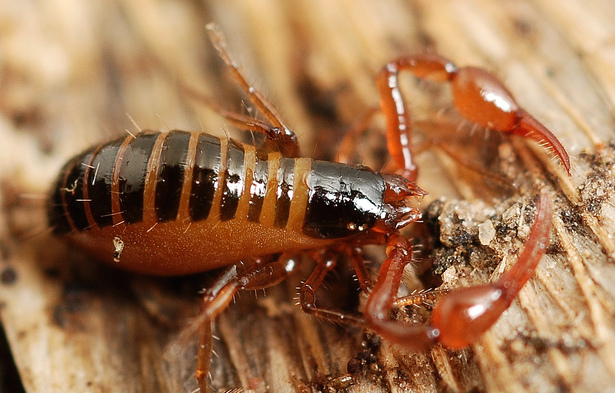
\includegraphics[width=0.7\textwidth]{pseudo}
  \caption{Pseudoscorpionida. Photo (CC BY-SA 2.0) by Gilles San Martin: \url{https://flic.kr/p/5Nxymf}}
  \label{fig:pseudo}
\end{figure}
\noindent{}Compared to the other arachnids we've seen, would you describe Pseudoscorpiones as being highly adapted for prey capture? What would you predict these arthropods eat?\vspace{2cm}

\noindent{}Did you see all the phenotypes listed above in the specimens we have? Which characters seem to be evolutionarily significant and why? \vspace{5cm}

\subsection{Myriapoda}
\begin{itemize}
\item antennae present as single pair
\item appendages uniramous (\textit{i.e.}, no branches)
\item mouthparts mandibulate (\textit{i.e.}, not chelicerate)
\end{itemize}

\subsubsection*{Diplopoda (millipedes)}
\begin{itemize}
\item most (apparent) segments with 2 pairs of legs (Figure \ref{fig:diplop2})
\item antennae usually 7-segmented, short
\item 30+ pairs of legs present usually
\item body usually round, tube-like; some species small, bristly (Figure \ref{fig:diplop1})
\end{itemize}

\begin{figure}[ht!]
    \centering
    \begin{subfigure}[ht!]{0.35\textwidth}
        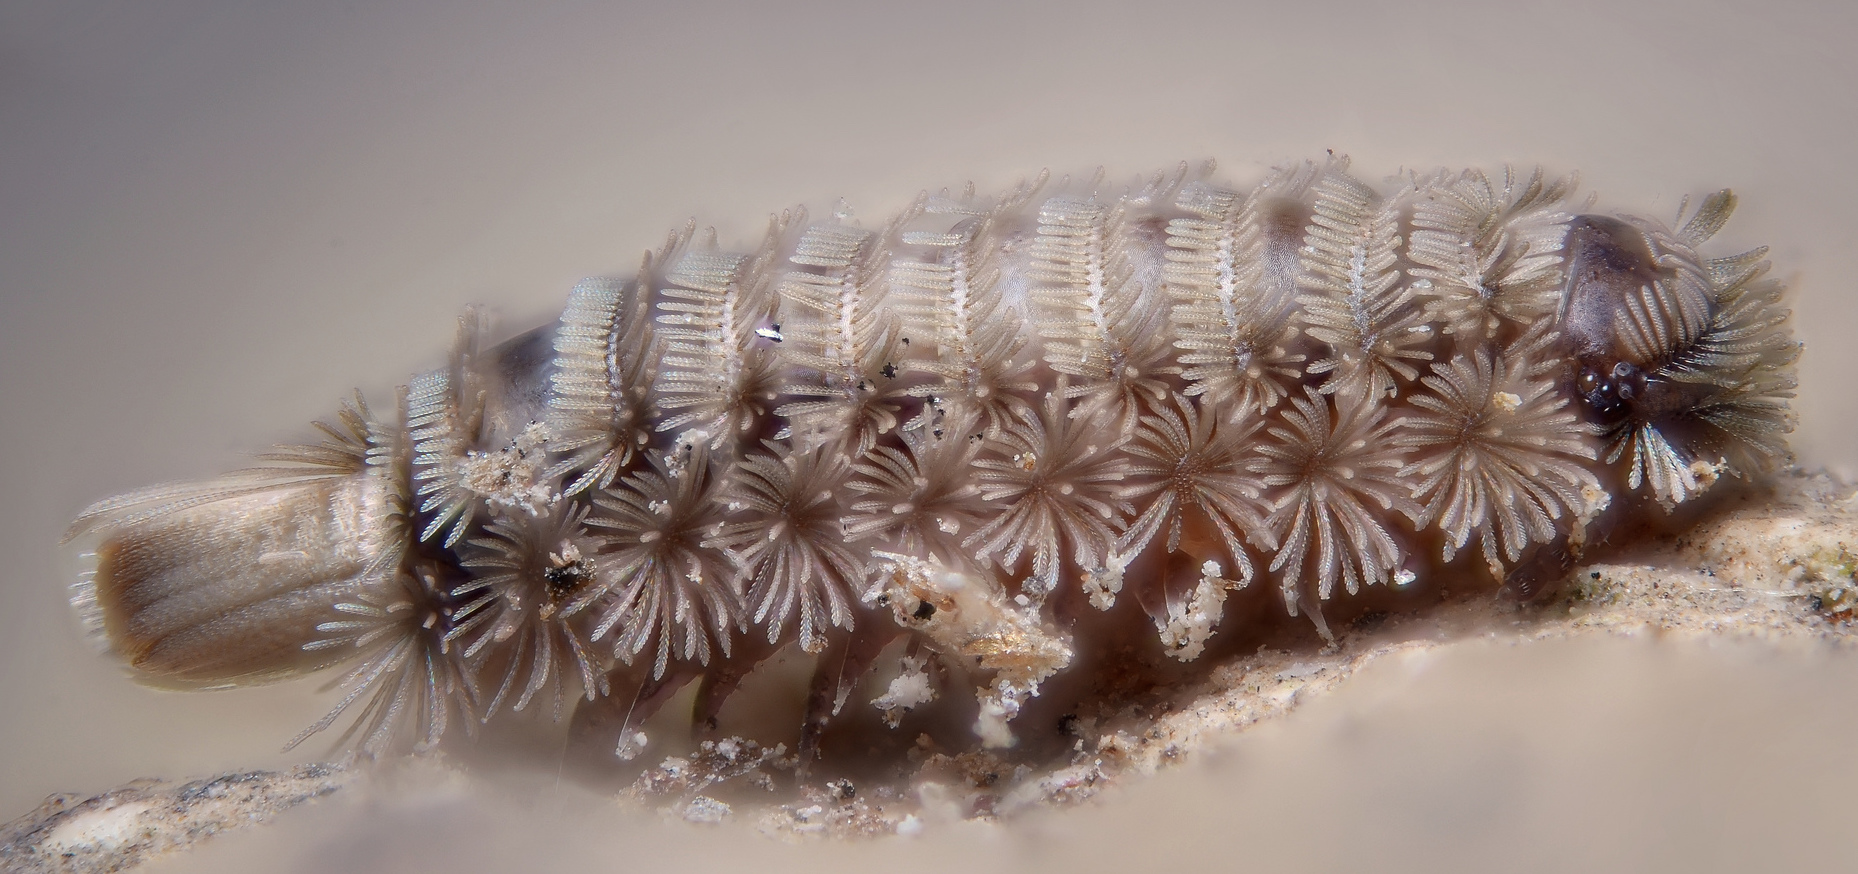
\includegraphics[width=\textwidth]{diplop1}
        \caption{Photo (CC BY 2.0) by Gilles San Martin: \url{https://flic.kr/p/dgF295}}
        \label{fig:diplop1}
    \end{subfigure}
    ~ %add desired spacing between images, e. g. ~, \quad, \qquad, \hfill etc. 
      %(or a blank line to force the subfigure onto a new line)
    \begin{subfigure}[ht!]{0.55\textwidth}
        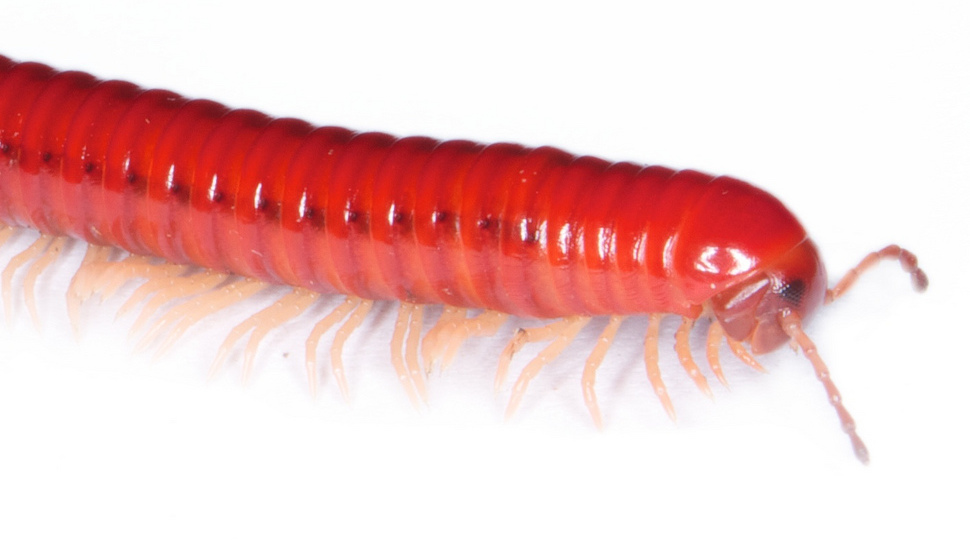
\includegraphics[width=\textwidth]{diplop2}
        \caption{Photo (CC BY 2.0) by Brian Gratwicke: \url{https://flic.kr/p/dFP5Wu}}
        \label{fig:diplop2}
    \end{subfigure}
    \caption{Millipedes (Diplopoda).} \label{fig:diplopoda}
\end{figure}

\subsubsection*{Chilopoda (centipedes)}
\begin{itemize}
\item antennae usually with 14+ segments
\item apices of anteriormost pair of legs (forcipules) modified into fang-like structures (Figure \ref{fig:chilo2})
\item most segments with 1 pair of legs; 15+ pairs of legs present usually (Figures \ref{fig:chilo1}--\ref{fig:chilo2})
\item body usually dorsoventrally flattened (but see Figure \ref{fig:chilo1})
\end{itemize}

\begin{figure}[ht!]
    \centering
        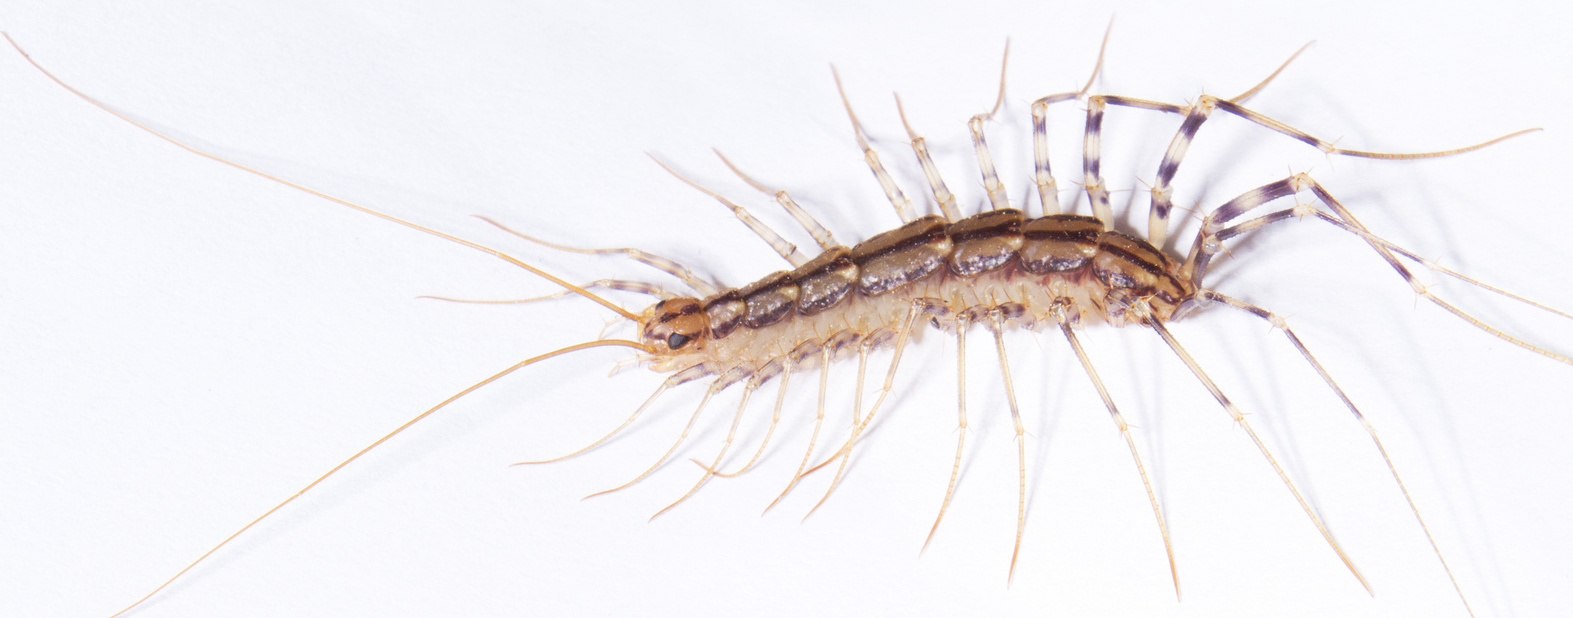
\includegraphics[width=0.7\textwidth]{chilo1}
        \caption{Chilopoda. Photo (CC BY 2.0) by Brian Gratwicke: \url{https://flic.kr/p/ehk44m}}
        \label{fig:chilo1}
\end{figure}

\begin{figure}[ht!]
	\centering
        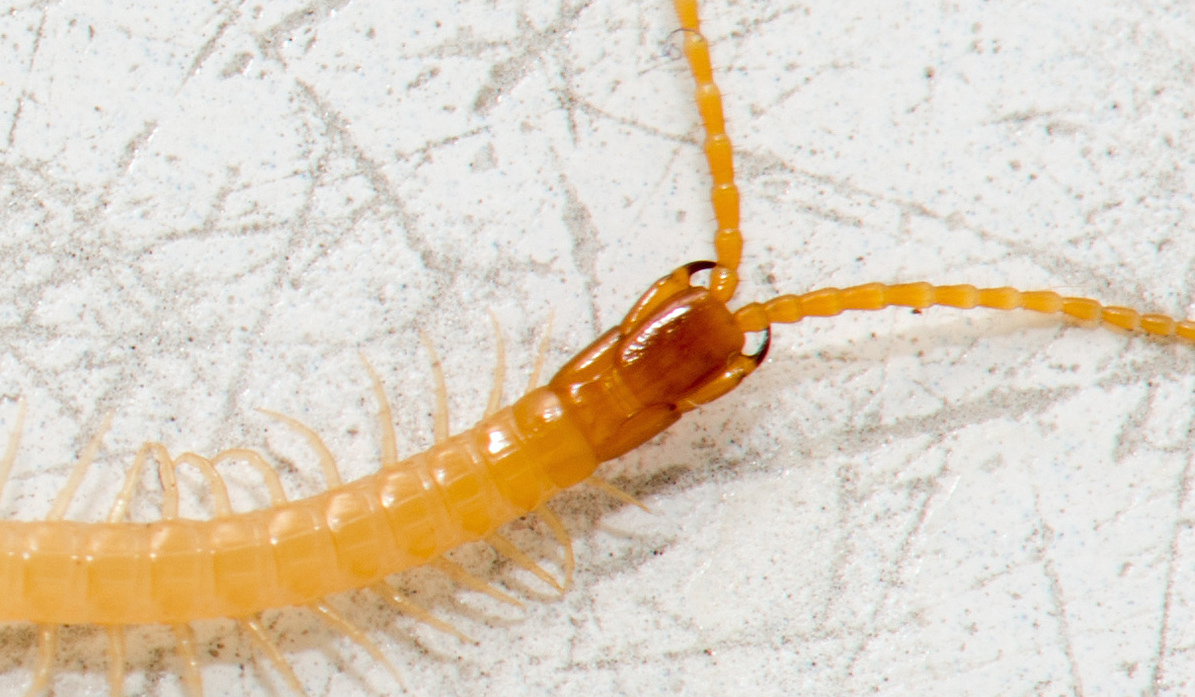
\includegraphics[width=0.7\textwidth]{chilo2}
        \caption{Chilopoda. Photo (CC BY 2.0) by Derrick Coetzee: \url{https://flic.kr/p/cF2Czu}}
        \label{fig:chilo2}
\end{figure}

\noindent{}Based on your observations of the two myriapod taxa we have in lab, what would you say about their natural history? Where does each taxon typically live, and what does it eat?\vspace{4cm}

\subsection{Non-hexapod Pancrustacea (formerly ``Crustacea'')}
\begin{itemize}
\item often with 2 tagmata: cephalothorax and abdomen
\item many biramous (2-branched) appendages, usually with 2nd pair of antennae (antennules)
\item mouthparts mandibulate
\end{itemize}

\subsubsection*{Isopoda (pillbugs, sowbugs)}
\begin{itemize}
\item body with no carapace, usually dorso-ventrally flattened (Figures \ref{fig:isopod1}--\ref{fig:isopod2})
\item 7 pairs of thoracic legs
\item 2nd pair of antennae reduced
\end{itemize}

\begin{figure}[ht!]
    \centering
    \begin{subfigure}[ht!]{0.55\textwidth}
        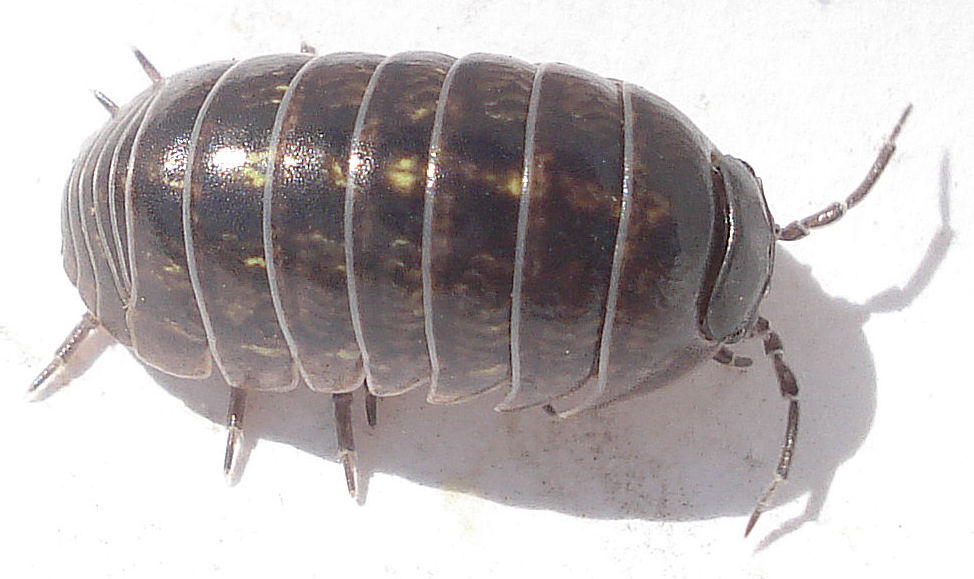
\includegraphics[width=\textwidth]{isopod}
        \caption{Photo (CC BY 2.0) by Mick Talbot \url{https://flic.kr/p/6vEqLt}}
        \label{fig:isopod1}
    \end{subfigure}
    ~ %add desired spacing between images, e. g. ~, \quad, \qquad, \hfill etc. 
      %(or a blank line to force the subfigure onto a new line)
    \begin{subfigure}[ht!]{0.35\textwidth}
        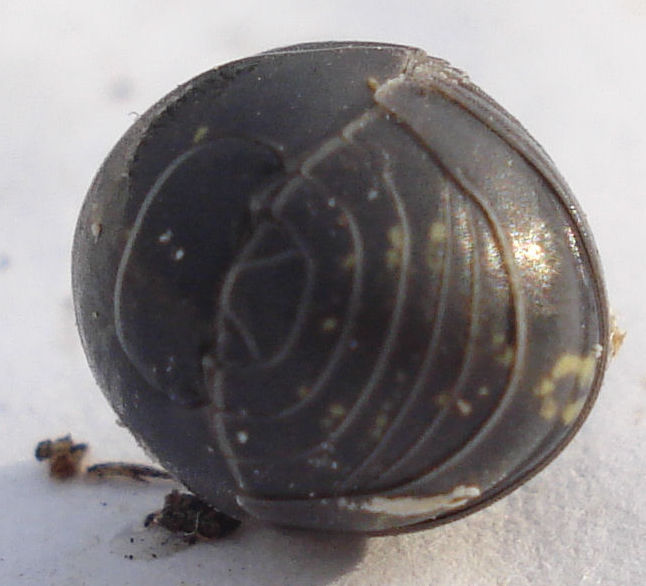
\includegraphics[width=\textwidth]{isopod2}
        \caption{Photo (CC BY 2.0) by Mick Talbot \url{https://flic.kr/p/6jQM1g}}
        \label{fig:isopod2}
    \end{subfigure}
    \caption{Isopoda} \label{fig:isopoda}
\end{figure}

\subsubsection*{Amphipoda (scuds)}
\begin{itemize}
\item no carapace, usually laterally flattened (Figure \ref{fig:amphip})
\item fore legs often raptorial
\item usually 6 or 7 pairs of thoracic legs
\end{itemize}

\begin{figure}[ht!]
  \centering
    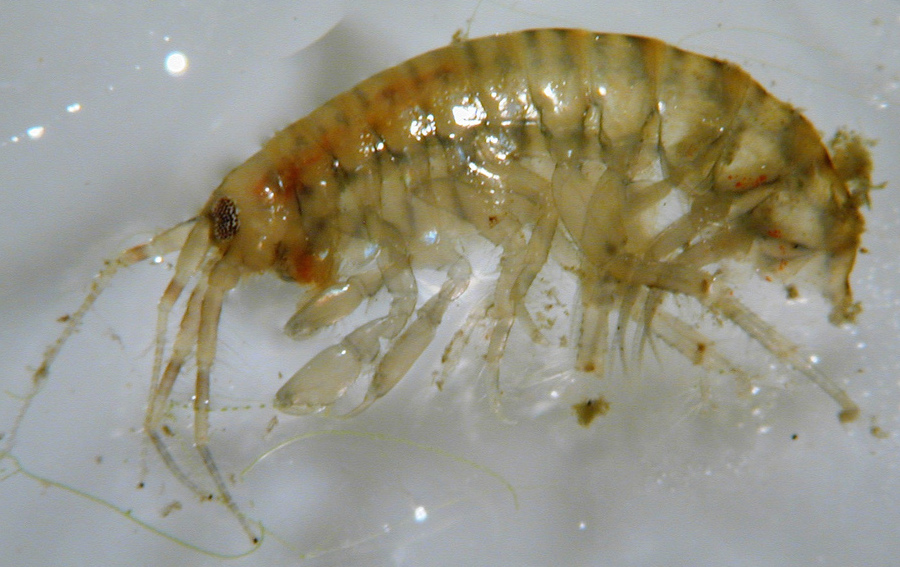
\includegraphics[width=0.65\textwidth]{amphip}
  \caption{Amphipoda. Photo (CC BY-NC 2.0) by Fred Snyder:  \url{https://flic.kr/p/9vTru1}}
  \label{fig:amphip}
\end{figure}

\noindent{}Given your observations of these ``crustaceans'', why do we have so few terrestrial and fresh water species, relative to insects? \vspace{3cm}

\subsection{Test your skills!}
You've now seen a handful of arthropod taxa, from three groups that are not insects. While they are not the focus of this course, these organisms are incredibly diverse and remain relevant to understanding the evolution of Arthropoda. Take some time to observe specimens of taxa we are not covering, bask in the diversity of phenotypes, and see if you can classify them correctly. Are the chelicerates, myriapods, or pancrustaceans? Why or why not? Draw and/or describe features you think are diagnostic. Based on their morphology, can you predict their natural history?

\subsubsection*{Solifugae (Solpugida; camelspiders, sunspiders, windscorpions)}
What group does it belong in and why?\vspace{1cm}

\noindent{}What diagnostic characters separate it from the taxa above?\vspace{1.5cm}

\noindent{}What do these arthropods eat, and how do they live?\vspace{1.5cm}

\begin{figure}[ht!]
  \centering
    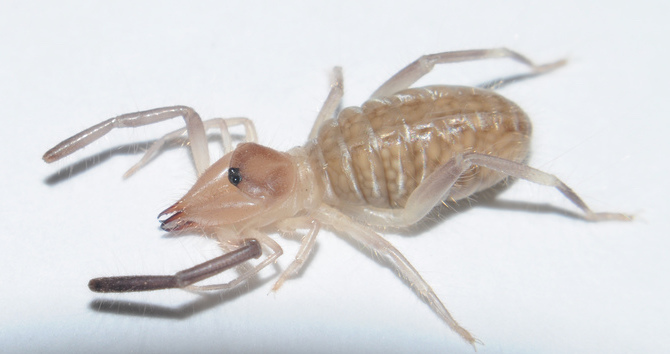
\includegraphics[width=0.6\textwidth]{solfugida}
  \caption{Solifugae. Photo (CC BY 2.0) by Maximilian Paradiz: \url{https://flic.kr/p/7J7B3r}}
  \label{fig:solfugida}
\end{figure}

\subsubsection*{Decapoda (crabs, lobsters, shrimp)}
What group does it belong in and why?\vspace{1cm}

\noindent{}What diagnostic characters separate it from the taxa above?\vspace{1.5cm}

\noindent{}What do these arthropods eat, and how do they live?\vspace{1.5cm}

\begin{figure}[ht!]
  \centering
    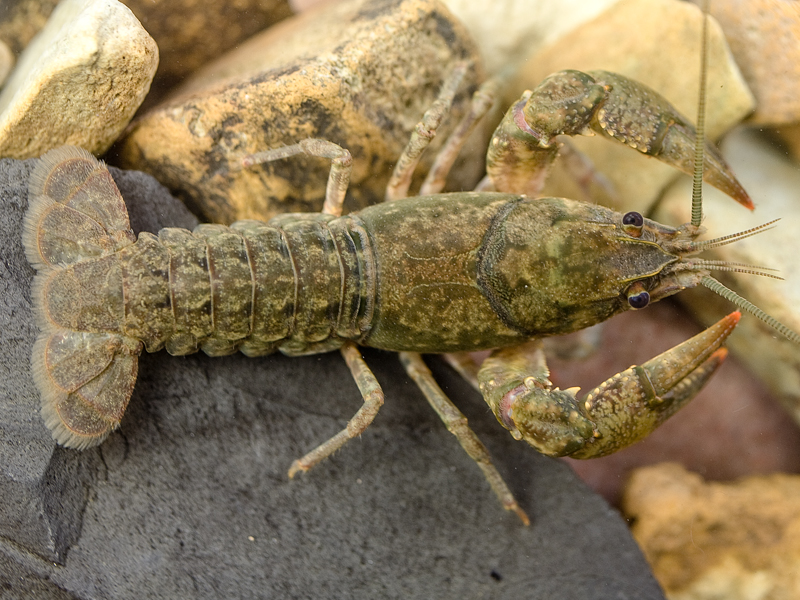
\includegraphics[width=0.6\textwidth]{decapod}
  \caption{Decapoda. Photo (CC BY 2.0) by Guenter Schuster: \url{https://flic.kr/p/njkdZ3}}.
  \label{fig:decapoda}
\end{figure}

\subsubsection*{Thelyphonida (Uropygi, Uropygida, vinegaroons, whipscorpions)}
What group does it belong in and why?\vspace{1cm}

\noindent{}What diagnostic characters separate it from the taxa above?\vspace{1.5cm}

\noindent{}What do these arthropods eat, and how do they live?\vspace{1.5cm}

\begin{figure}[ht!]
  \centering
    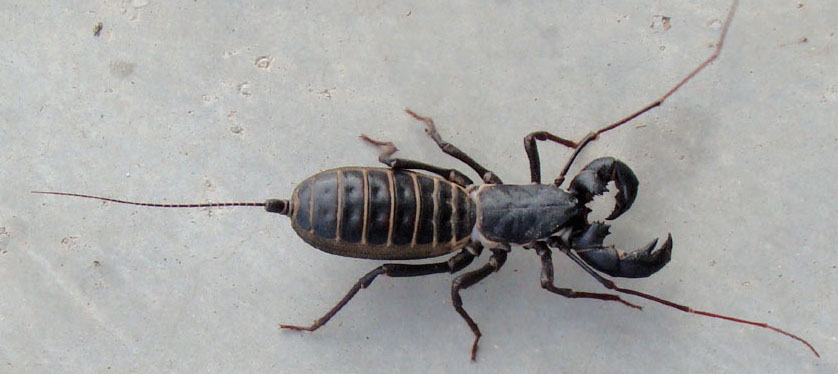
\includegraphics[width=0.6\textwidth]{thelyphonida}
  \caption{Thelyphonida. Photo (CC BY-NC-SA 2.0) by StarWatcher307: \url{https://flic.kr/p/8hde2g}}
  \label{fig:thelyphonida}
\end{figure}

\subsubsection*{Amblypygi (tail-less whipscorpions)}
What group does it belong in and why?\vspace{1cm}

\noindent{}What diagnostic characters separate it from the taxa above?\vspace{1.5cm}

\noindent{}What do these arthropods eat, and how do they live?\vspace{1.5cm}

\begin{figure}[ht!]
  \centering
    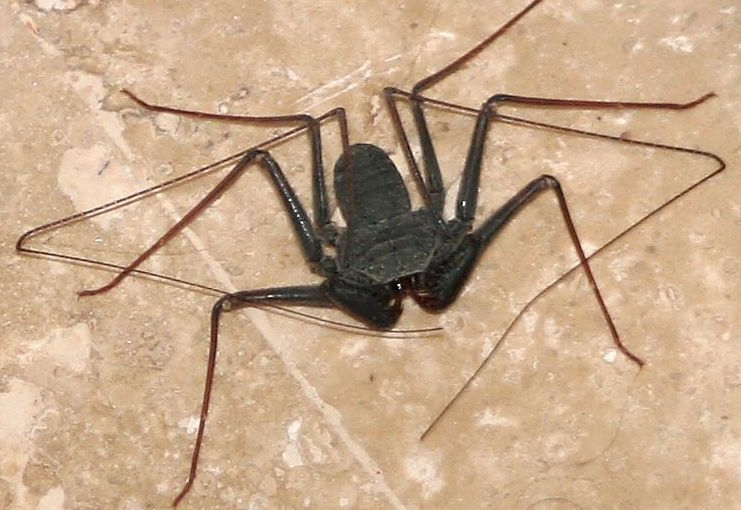
\includegraphics[width=0.6\textwidth]{ambly1}
  \caption{Amblypygi. Photo (CC BY-NC-SA 2.0) by Jos\'{e} Eugenio G\'{o}mez Rodr\'{i}guez: \url{https://flic.kr/p/5hmWNS} }
  \label{fig:ambly1}
\end{figure}

\subsubsection*{Xiphosura (horseshoe crabs)}
What group does it belong in and why?\vspace{1cm}

\noindent{}What diagnostic characters separate it from the taxa above?\vspace{1.5cm}

\noindent{}What do these arthropods eat, and how do they live?\vspace{1.5cm}

\begin{figure}[ht!]
  \centering
    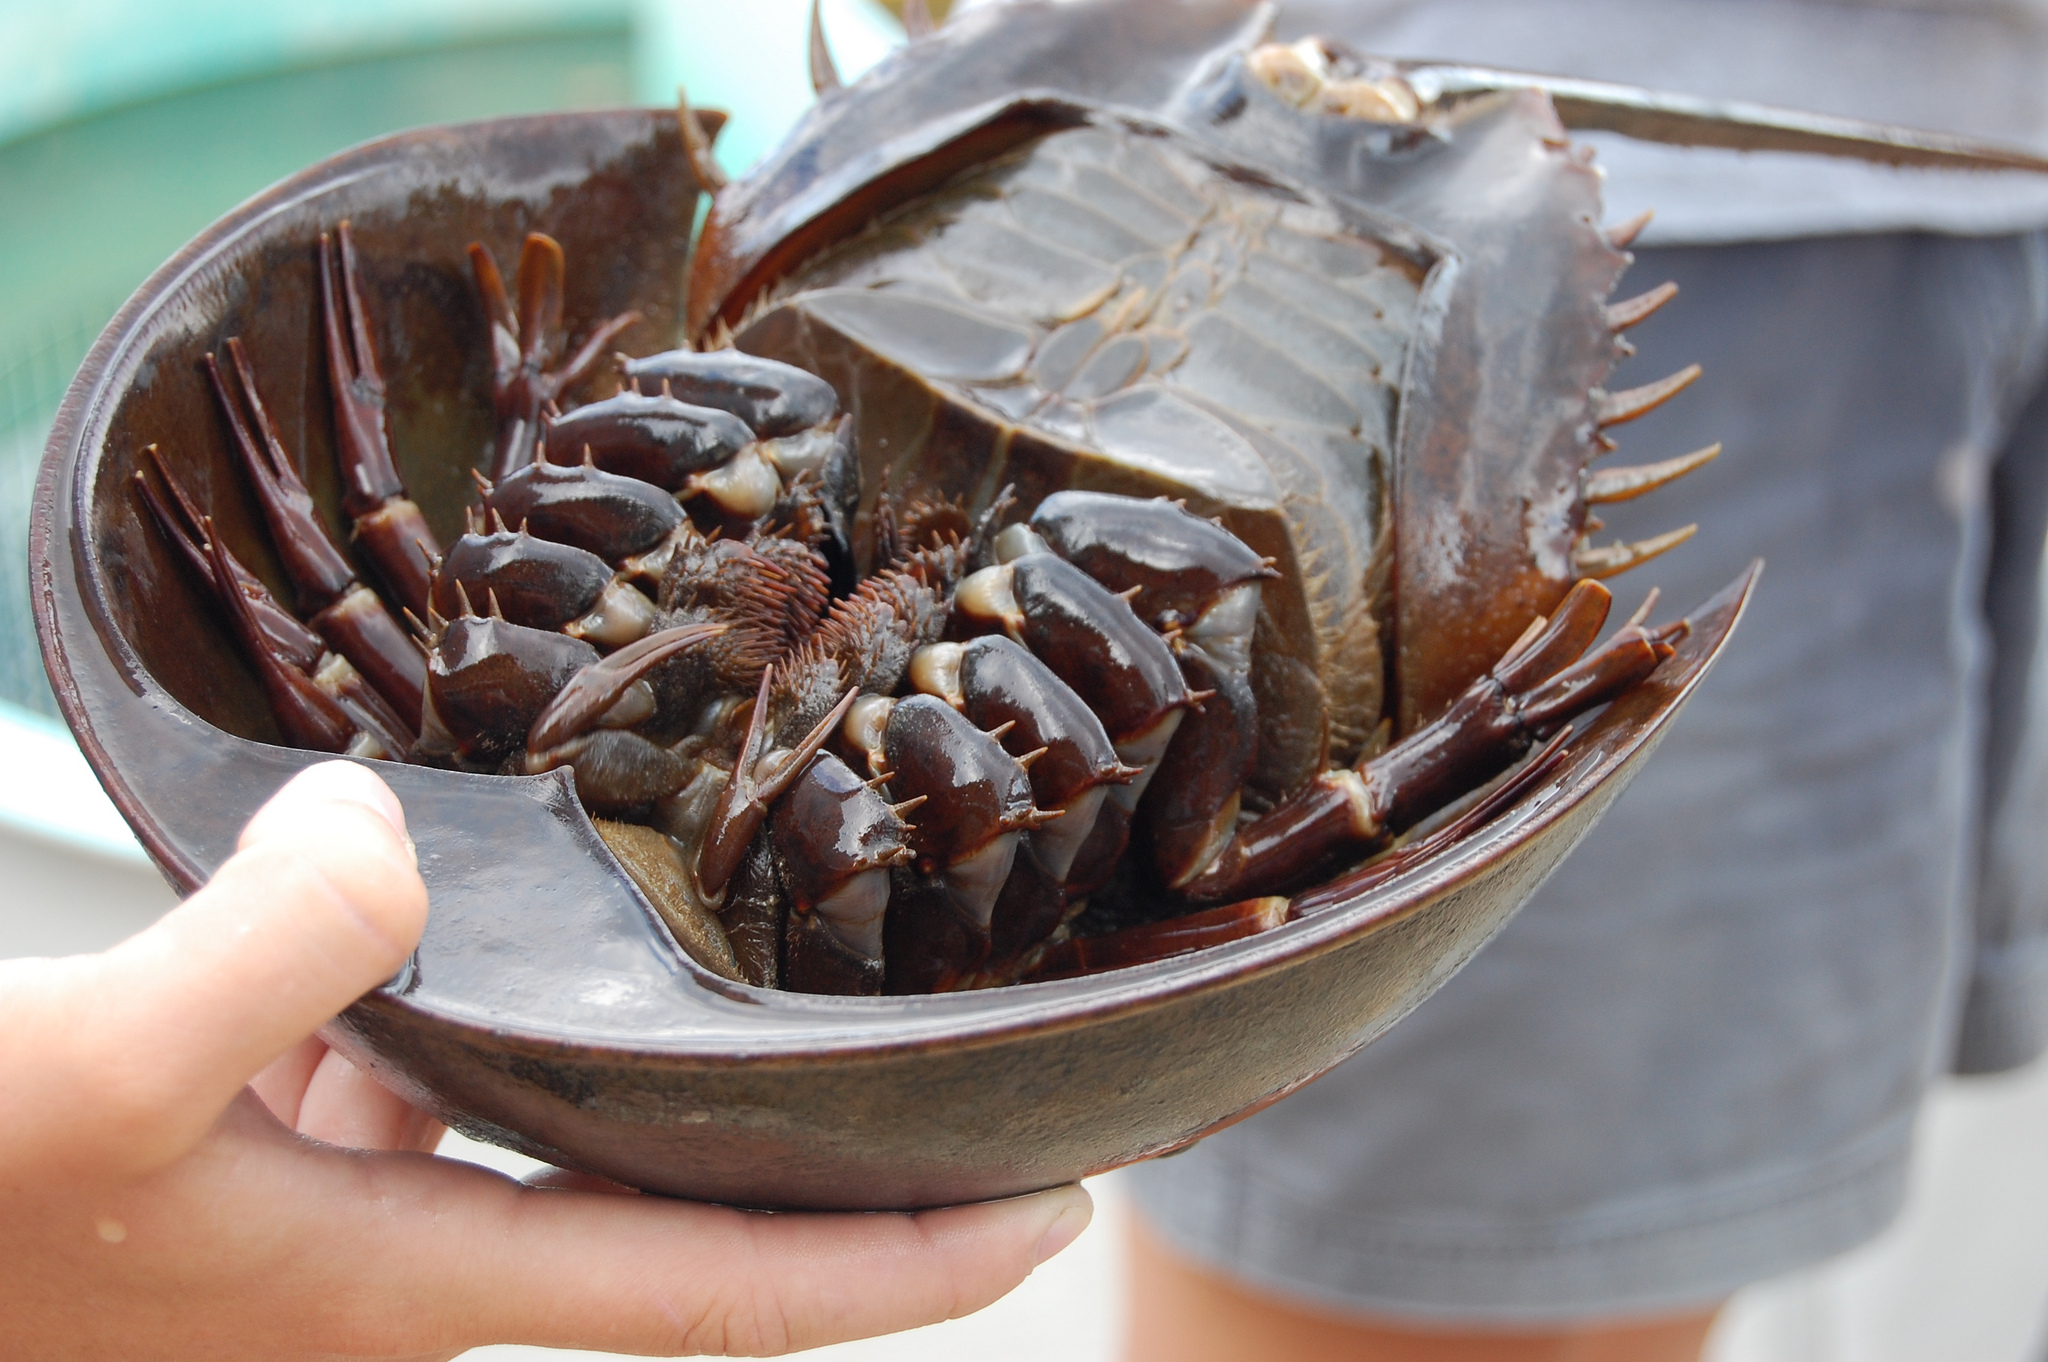
\includegraphics[width=0.6\textwidth]{xipho}
  \caption{Xiphosura. Photo (CC BY-ND 2.0) NH Sea Grant: https://flic.kr/p/duEyis: \url{https://flic.kr/p/85z27d}}.
  \label{fig:xipho}
\end{figure}

\subsubsection*{Copepoda (copepods, fish lice)}
What group does it belong in and why?\vspace{1cm}

\noindent{}What diagnostic characters separate it from the taxa above?\vspace{1.5cm}

\noindent{}What do these arthropods eat, and how do they live?\vspace{1.5cm}

\begin{figure}[ht!]
  \centering
    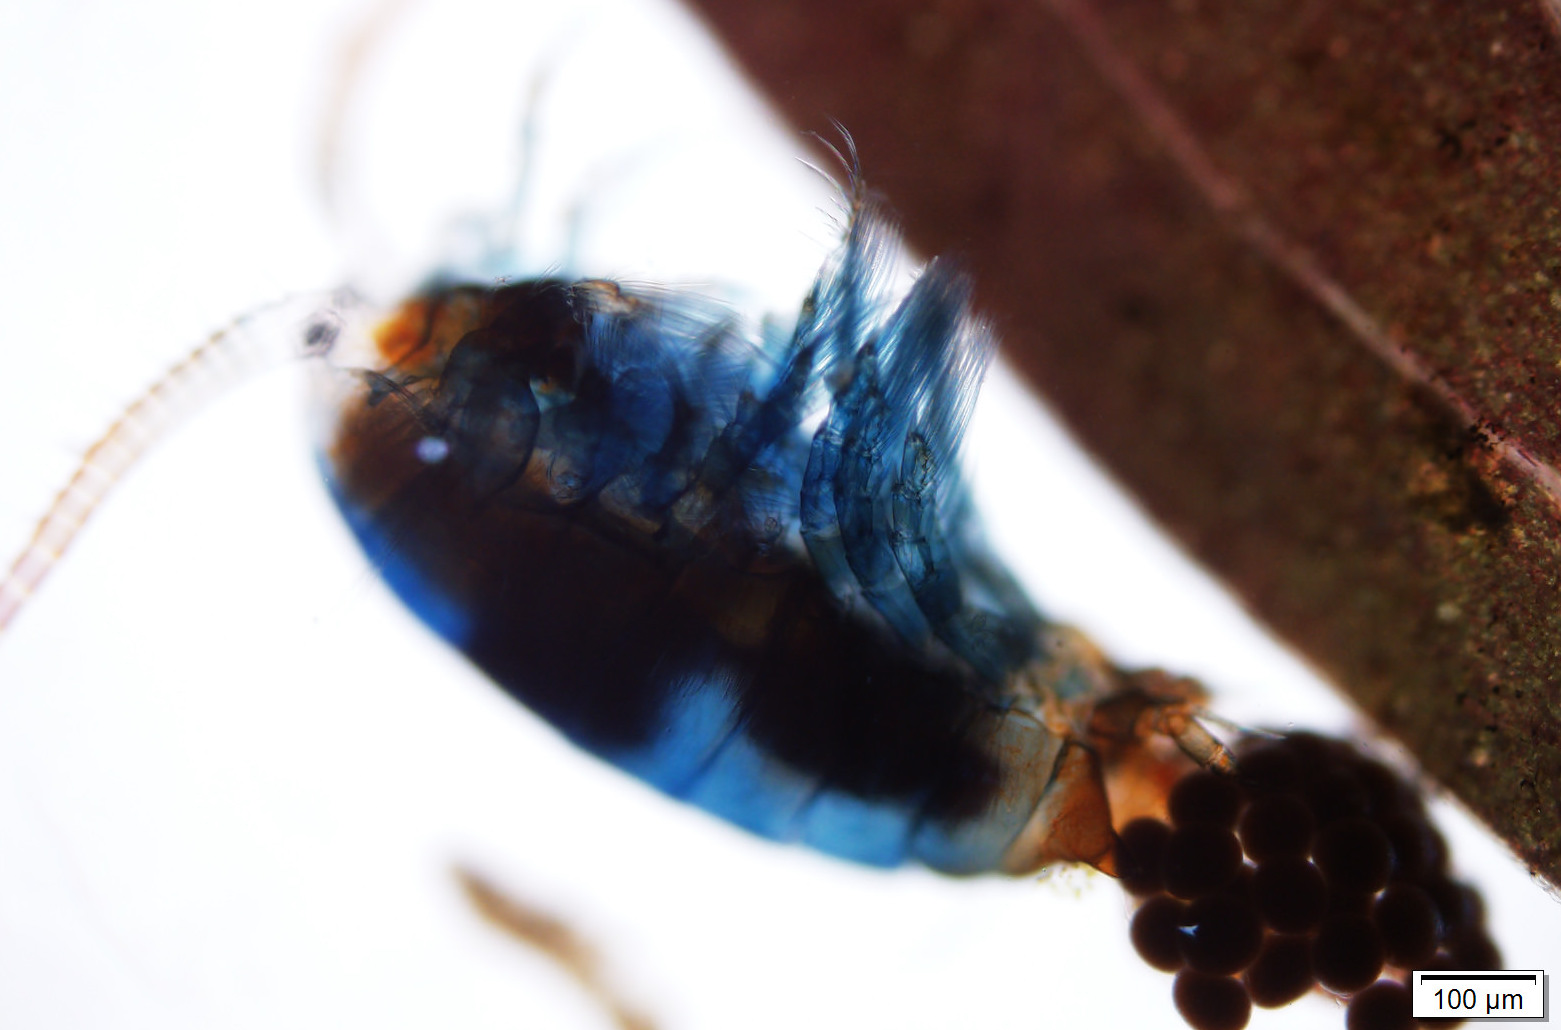
\includegraphics[width=0.6\textwidth]{copepod}
  \caption{Copepod from Ten Acre Pond (Centre Co., Pennsylvania). Photo (CC BY 2.0) by Andy Deans: \url{https://flic.kr/p/nsJuJZ}}
  \label{fig:copepod}
\end{figure}


\subsubsection*{Symphyla (symphylans)}
What group does it belong in and why?\vspace{1cm}

\noindent{}What diagnostic characters separate it from the taxa above?\vspace{1.5cm}

\noindent{}What do these arthropods eat, and how do they live?\vspace{1.5cm}

\begin{figure}[ht!]
  \centering
    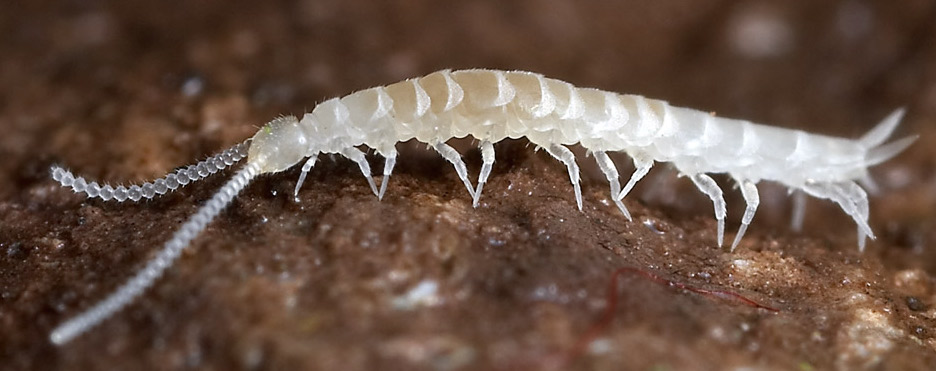
\includegraphics[width=0.6\textwidth]{Symphyla}
  \caption{Symphyla. Photo (CC BY-SA 3.0) by Sonia Martinez: \url{http://bit.ly/1iRxA29}}
  \label{fig:symphyla}
\end{figure}

\begin{thebibliography}{9} %expand?
\bibitem{terrest} Greb, S. F., W. A. DiMichele, and R. A. Gastaldo (2006) Evolution and importance of wetlands in earth history. Geological Society of America Special Papers, 399:1--40 DOI: 10.1130/2006.2399(01)
\bibitem{review} Dunlop, J. A. (2010) Geological history and phylogeny of Chelicerata. Arthropod Structure \& Development, 39(2--3):124--142 DOI: 10.1016/j.asd.2010.01.003. Fossil Record and Phylogeny of the Arthropoda.
\bibitem{syllabus} Miyazawa, H., C. Ueda, K. Yahata, and Z.-H. Su. (2010) Molecular phylogeny of Myriapoda provides insights into evolutionary patterns of the mode in post-embryonic development. \textit{Scientic Reports}, 4(4127):1--9 DOI: 10.1038/srep04127.
\end{thebibliography}

\end{document}